\documentclass[a4paper, 14pt, titlepage, fleqn]{extarticle}
\usepackage{style}
\usepackage{mathrsfs}
\usepackage{float}
\usepackage{indentfirst}
\usepackage{setspace}
\usepackage{indentfirst}
\usepackage{pythonhighlight}
\setmainfont{Times New Roman}
\DeclareMathOperator{\erfi}{erfi}






\begin{document}
	\fefutitlepage{ОТЧЕТ}{к лабораторной работе №1\\по дисциплине <<Дифференциальные уравнения и теоретическая механика>>}{02.03.01 <<Математика и компьютерные науки>>}{Б9120-02.03.01 сцт}{Пограничный К.О.}
	\setcounter{page}{2}
	\tableofcontents
	\setlength{\baselineskip}{25pt}
	\newpage

	\onehalfspacing

%	\addcontentsline{toc}{section}{\hyperlink{Введение}{Введение}}
%	\hypertarget{Введение}{\section*{Введение}}

		\phantomsection
		\sect{Введение}

		В данной лабораторной работе необходимо реализовать алгоритм постро-
        ения интегрального преобразования Фурье для произвольно заданных функ-
        ций одной переменной. Построить графики, основанные на данных, получен-
        ных при самостоятельном и при программном поиске преобразования заданной
        функции.
	\pagebreak

	\begin{specialx}
	\section{Задание}
		\subsection{Постановка задачи}

			Задана произвольная функция одной переменной. Реализация производится с помощью численных методов расчета интегралов. Требуется построить график функции  \(f(t)\) и её вещественные спектральные разложения.\\Для реализации потребуются следующие параметры:

			\begin{itemize}
				\item \(f(t)\) -- определение функции,
				\item \(a,b\) -- область интегрирования функции,
				\item \(n_1\) -- количество разбиений области интегрирования,
				\item \(n_2	\) -- количество разбиений частотного диапазона,
				\item \(m\) -- максимальное значение частоты.
			\end{itemize}

			Задача сводится к построению спектрального разложения одномерного сигнала \(f(t)\) на частоты составляющих его волн.

                Реализация проводится с помощью численных методов расчета
            интегралов. Потребуется построить график функции \(f(t)\), и ее вещественные и комплексные спектральные разложения (\(\mathscr{F_{\Re}}\{f\}\) и \(\mathscr{F_{\Im}}\{f\}\)).
			Оси графиков
			разложений представляют из себя по горизонтали -- частотный диапазон, по вертикали -- амплитуда.

			Решение оформить в среде \LaTeX.

	\section{Решение}
            \subsection{Теория}
			Интегральное преобразование Фурье определяется следующим образом:\\
				$$F(f(t)=\int_{-\infty}^{+\infty}{e^{-2\pi \omega t i }}f\left(t \right)= (\omega )$$

                Вещественное (косинус) преобразование Фурье определяется как:
                $$F_{R}\left\{{f(t)} \right\}=\int_{-\infty}^{+\infty}{cos(2\pi \omega t)} \cdot f\left(t \right)dt$$
                Комплексное (синус) преобразование Фурье определяется как:
                $$F_{I}\left\{{f(t)} \right\}=\int_{-\infty}^{+\infty}{sin(2\pi \omega t)} \cdot f\left(t \right)dt$$\\

            \subsection{Вычисление значения функции}
                Рассмотрим функцию \(f\left(t \right)=\sin \left(\sqrt{t} \right)e^{-t}\) на диапазоне \([a, b] = [0, \pi^2]\), в остальном диапазоне полагая \(f(t) = 0\). Для аналитического решения, функция примет вид: \(f\left(t \right)=\sin \left(\sqrt{t} \right) e^{-t} \cdot \Pi_{0,\pi^2}\left(t\right) \). Положим \( \chi = 2\pi\omega \). Тогда преобразование Фурье примет вид:
				$$\mathscr{F}\left\{\sin \left(\sqrt{t} \right)e^{-t}\right\}
				& = \int\displaylimits_{-\infty}^{\infty} \sin \left(\sqrt{t} \right)e^{-t} \cdot e^{-i\chi t} \cdot \Pi_{0,\pi^2}~dt
                & = \int\displaylimits_{0}^{\pi^2} \sin \left(\sqrt{t} \right)e^{-t} \cdot e^{-i\chi t}~dt$$

                 Вещественные и комплексные спектральные разложения (\(\mathscr{F_{\Re}}\{f\left(t \right)\}\) и\\ \(\mathscr{F_{\Im}}\{f\left(t \right)\}\)) примут следующий вид:

                 \begin{align*}
				&\mathscr{F_{\Re}}\{\sin \left(\sqrt{t}\right)e^{-t}\} = \int\displaylimits_{-\infty}^{\infty} \sin \left(\sqrt{t} \right)e^{-t} \cdot \cos(\chi t) \cdot \Pi_{0,\pi^2}~dt =\\ &= \int\displaylimits_{0}^{\pi^2} \sin \left(\sqrt{t} \right)e^{-t}\ \cdot \cos(\chi t)~dt = (*)\\
                        & \left| \begin{array}{c}
                            & t = \tau^2 \\
                            & ~dt = 2 \tau ~d\tau \\
                        \end{array}\right|\\
                    & (*) = 2\cdoc\int\displaylimits_{0}^{\pi^2} \tau e^{-\tau^{2}} \sin(\tau) \cdot \cos(\chi \tau^2)~d\tau = \\
                    &= -\dfrac{i}{2}\int\displaylimits_{0}^{\pi^2}\tau (e^{i\tau} - e^{-i\tau})e^{-\tau^{2}}\cdoc (e^{i \chi \tau^{2}} + e^{-i \chi \tau^{2}})~d\tau = \\
                    &= -\dfrac{i}{2}\int\displaylimits_{0}^{\pi^2}\tau e^{i\chi\tau^{2}-\tau^{2}+i\tau}~d\tau + \dfrac{i}{2}\int\displaylimits_{0}^{\pi^2}\tau e^{i\chi\tau^{2}-\tau^{2}-i\tau}~d\tau - \\
                    &-\dfrac{i}{2}\int\displaylimits_{0}^{\pi^2}\tau e^{-i\chi\tau^{2}-\tau^{2}+i\tau}~d\tau + \dfrac{i}{2}\int\displaylimits_{0}^{\pi^2}\tau e^{-i\chi\tau^{2}-\tau^{2}-i\tau}~d\tau\ =\\\\
                    &= -\dfrac{i}{2}\left(\dfrac{e^{i\chi\tau^{2}-\tau^{2}+i\tau}}{2\left(i\chi-1\right)}-\dfrac{\sqrt{\pi}ie^{\frac{1}{4\left(i\chi-1\right)}}\erfi\left(\dfrac{2\left(i\chi-1\right)\tau+i}{2\sqrt{i\chi-1}}\right)}{4\left(i\chi-1\right)^{\frac{3}{2}}}\right) +\\\\
                    & + \dfrac{i}{2}\left(\dfrac{e^{i\chi\tau^{2}-\tau^{2}-i\tau}}{2\left(i\chi-1\right)}-\dfrac{\sqrt{\pi}ie^{\frac{1}{4\left(i\chi-1\right)}}\erfi\left(\dfrac{2\left(i\chi-1\right)\tau-i}{2\sqrt{i\chi-1}}\right)}{4\left(i\chi-1\right)^{\frac{3}{2}}}\right) -\\
                    \end{align*}
                    \begin{align*}
                    & -\dfrac{i}{2}\left(\dfrac{\sqrt{\pi}ie^{-\frac{1}{4\left(i\chi+1\right)}}\erfi\left(\dfrac{2\left(-i\chi-1\right)\tau+i}{2\sqrt{-i\chi-1}}\right)}{4\sqrt{-i\chi-1}\left(i\chi+1\right)} - \dfrac{e^{-i\chi\tau^{2}-\tau^{2}+i\tau}}{2\left(i\chi+1\right)}\right) -\\\\
                    & -\dfrac{i}{2}\left(\dfrac{\sqrt{\pi}i e^{-\frac{1}{4\left(i\chi+1\right)}}\erfi\left(\dfrac{2\left(-i\chi-1\right)\tau-i}{2\sqrt{-i\chi-1}}\right)}{4\sqrt{-i\chi-1}\left(i\chi+1\right)} + \dfrac{e^{-i\chi\tau^{2}-\tau^{2}-i\tau}}{2\left(i\chi+1\right)}\right) = (*)\\\\
                    &\text{Раскроем скобки и сделаем обратную замену:}\\\\
                    &(*) = -\dfrac{ie^{i\chi t - t + i \sqrt{t}}}{4\left(i\chi-1\right)} + \dfrac{ie^{i\chi t - t - i \sqrt{t}}}{4\left(i\chi-1\right)} + \dfrac{ie^{-i\chi t - t + i \sqrt{t}}}{4\left(i\chi+1\right)} - \dfrac{ie^{-i\chi t - t - i \sqrt{t}}}{4\left(i\chi+1\right)} -\\\\
                    & -\dfrac{\sqrt{\pi}e^{\frac{1}{4\left(i\chi-1\right)}}\erfi\left(\dfrac{2\left(i\chi-1\right)\sqrt{t}+i}{2\sqrt{i\chi-1}}\right)}{8\left(i\chi-1\right)^\frac{3}{2}} -\\\\
                    & -\dfrac{\sqrt{\pi}e^{\frac{1}{4\left(i\chi-1\right)}}\erfi\left(\dfrac{2\left(i\chi-1\right)\sqrt{t}-i}{2\sqrt{i\chi-1}}\right)}{8\left(i\chi-1\right)^\frac{3}{2}} +\\\\
                    & +\dfrac{\sqrt{\pi}e^{-\frac{1}{4\left(i\chi+1\right)}}\erfi\left(\dfrac{2\left(-i\chi-1\right)\sqrt{t}+i}{2\sqrt{-i\chi-1}}\right)}{8\sqrt{-i\chi-1}\left(i\chi+1\right)} +\\\\
                    & +\dfrac{\sqrt{\pi}e^{-\frac{1}{4\left(i\chi+1\right)}}\erfi\left(\dfrac{2\left(-i\chi-1\right)\sqrt{t}-i}{2\sqrt{-i\chi-1}}\right)}{8\sqrt{-i\chi-1}\left(i\chi+1\right)},\\\\
                    &\text{где } \textsl{erfi(x)} \text{ - функция ошибок.}\\
                \end{align*}
                \begin{align*}
				&\mathscr{F_{\Im}}\{\sin \left(\sqrt{t}\right)e^{-t}\} = \int\displaylimits_{-\infty}^{\infty} \sin \left(\sqrt{t} \right)e^{-t} \cdot \sin(\chi t) \cdot \Pi_{0,\pi^2}~dt =\\ &= \int\displaylimits_{0}^{\pi^2} \sin \left(\sqrt{t} \right)e^{-t}\ \cdot \sin(\chi t)~dt = (*)\\
                        & \left| \begin{array}{c}
                            & t = \tau^2 \\
                            & ~dt = 2 \tau ~d\tau \\
                        \end{array}\right|\\
                    & (*) = 2\cdoc\int\displaylimits_{0}^{\pi^2} \tau e^{-\tau^{2}} \sin(\tau) \cdot \sin(\chi \tau^2)~d\tau = \\
                    &= -\dfrac{1}{2}\int\displaylimits_{0}^{\pi^2}\tau (e^{i\tau} - e^{-i\tau})e^{-\tau^{2}}\cdoc (e^{i \chi \tau^{2}} - e^{-i \chi \tau^{2}})~d\tau = \\
                    &= -\dfrac{1}{2}\int\displaylimits_{0}^{\pi^2}\tau e^{i\chi\tau^{2}-\tau^{2}+i\tau}~d\tau + \dfrac{1}{2}\int\displaylimits_{0}^{\pi^2}\tau e^{i\chi\tau^{2}-\tau^{2}-i\tau}~d\tau + \\
                    &+\dfrac{1}{2}\int\displaylimits_{0}^{\pi^2}\tau e^{-i\chi\tau^{2}-\tau^{2}+i\tau}~d\tau - \dfrac{1}{2}\int\displaylimits_{0}^{\pi^2}\tau e^{-i\chi\tau^{2}-\tau^{2}-i\tau}~d\tau\ =\\\\
                    &= -\dfrac{1}{2}\left(\dfrac{e^{i\chi\tau^{2}-\tau^{2}+i\tau}}{2\left(i\chi-1\right)}-\dfrac{\sqrt{\pi}ie^{\frac{1}{4\left(i\chi-1\right)}}\erfi\left(\dfrac{2\left(i\chi-1\right)\tau+i}{2\sqrt{i\chi-1}}\right)}{4\left(i\chi-1\right)^{\frac{3}{2}}}\right) +\\\\
                    & + \dfrac{1}{2}\left(\dfrac{e^{i\chi\tau^{2}-\tau^{2}-i\tau}}{2\left(i\chi-1\right)}+\dfrac{\sqrt{\pi}ie^{\frac{1}{4\left(i\chi-1\right)}}\erfi\left(\dfrac{2\left(i\chi-1\right)\tau-i}{2\sqrt{i\chi-1}}\right)}{4\left(i\chi-1\right)^{\frac{3}{2}}}\right) +\\
                    \end{align*}
                    \begin{align*}
                    & +\dfrac{1}{2}\left(\dfrac{\sqrt{\pi}ie^{-\frac{1}{4\left(i\chi+1\right)}}\erfi\left(\dfrac{2\left(-i\chi-1\right)\tau+i}{2\sqrt{-i\chi-1}}\right)}{4\sqrt{-i\chi-1}\left(i\chi+1\right)} - \dfrac{e^{-i\chi\tau^{2}-\tau^{2}+i\tau}}{2\left(i\chi+1\right)}\right) +\\\\
                    & +\dfrac{1}{2}\left(\dfrac{\sqrt{\pi}i e^{-\frac{1}{4\left(i\chi+1\right)}}\erfi\left(\dfrac{2\left(-i\chi-1\right)\tau-i}{2\sqrt{-i\chi-1}}\right)}{4\sqrt{-i\chi-1}\left(i\chi+1\right)} + \dfrac{e^{-i\chi\tau^{2}-\tau^{2}-i\tau}}{2\left(i\chi+1\right)}\right) = (*)\\\\
                    &\text{Раскроем скобки и сделаем обратную замену:}\\\\
                    &(*) = -\dfrac{e^{i\chi t - t + i \sqrt{t}}}{4\left(i\chi-1\right)} + \dfrac{e^{i\chi t - t - i \sqrt{t}}}{4\left(i\chi-1\right)} - \dfrac{e^{-i\chi t - t + i \sqrt{t}}}{4\left(i\chi+1\right)} + \dfrac{e^{-i\chi t - t - i \sqrt{t}}}{4\left(i\chi+1\right)} +\\\\
                    & +\dfrac{\sqrt{\pi}ie^{\frac{1}{4\left(i\chi-1\right)}}\erfi\left(\dfrac{2\left(i\chi-1\right)\sqrt{t}+i}{2\sqrt{i\chi-1}}\right)}{8\left(i\chi-1\right)^\frac{3}{2}} +\\\\
                    & +\dfrac{\sqrt{\pi}ie^{\frac{1}{4\left(i\chi-1\right)}}\erfi\left(\dfrac{2\left(i\chi-1\right)\sqrt{t}-i}{2\sqrt{i\chi-1}}\right)}{8\left(i\chi-1\right)^\frac{3}{2}} +\\\\
                    & +\dfrac{\sqrt{\pi}ie^{-\frac{1}{4\left(i\chi+1\right)}}\erfi\left(\dfrac{2\left(-i\chi-1\right)\sqrt{t}+i}{2\sqrt{-i\chi-1}}\right)}{8\sqrt{-i\chi-1}\left(i\chi+1\right)} +\\\\
                    & +\dfrac{\sqrt{\pi}ie^{-\frac{1}{4\left(i\chi+1\right)}}\erfi\left(\dfrac{2\left(-i\chi-1\right)\sqrt{t}-i}{2\sqrt{-i\chi-1}}\right)}{8\sqrt{-i\chi-1}\left(i\chi+1\right)},\\\\
                    &\text{где } \textsl{erfi(x)} \text{ - функция ошибок.}\\
                \end{align*}


            \subsection{Построение графиков}
            После произведенных преобразований функции  \(f\left(t \right)=\sin \left(\sqrt{t} \right)e^{-t}\) на диапазоне \([a, b] = [0, \pi^2]\), предполагая в остальном диапозоне \(f(t) = 0\), построим её спектральный график в аналитической и численной формах.

           \begin{figure}[H]
				\centering
				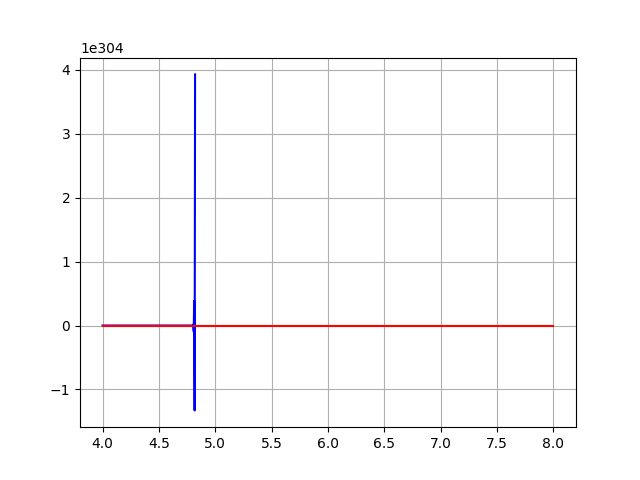
\includegraphics[width = 0.6\linewidth]{assets/myplot_1.png}
				\caption[.] {Спектральный график волн синус- и косинус-преобразований (синий --     вещественное преобразование, красный -- комплексное преобразование)}
			\end{figure}

			В процессе реализации численного алгоритма, минимальное значение частоты выберем \(m_{min} = 4\), а максимальное значение - \(m_{max} = 10\). Таким образом, численно найденный спектральный график имеет вид:
			\begin{figure}[H]
				\centering
				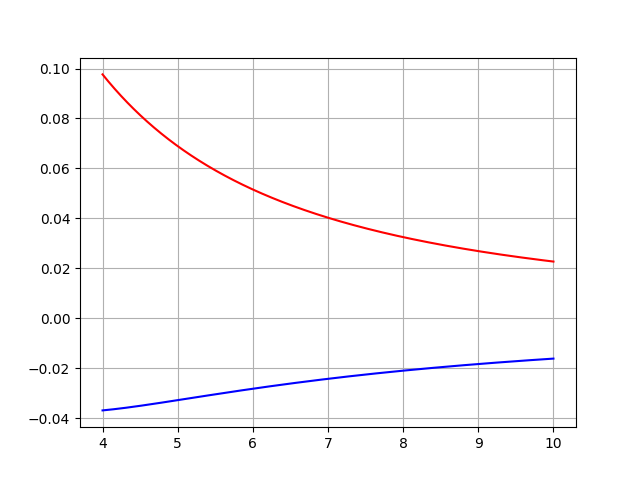
\includegraphics[width = 0.75\linewidth]{assets/myplot_2.png}
				\caption[.] {Численно рассчитанный спектральный график волн синус- и косинус- преобразований (красный -- комплексное преобразование, синий -- вещественное)}
			\end{figure}
	\pagebreak

\phantomsection

  \section{Приложение}
  Для написания алгоритма, реализующего преобразование Фурье, использовался язык программирования Python. В написанной программе реализована функция, вычисляющая действительную и мнимую части интегрального преобразования Фурье, а также осуществляется вывод полученных результатов в виде графиков.
  \subsection{Листинг программы}
  \begin{python}

import numpy as np
import matplotlib.pyplot as plt
import math
from scipy import special
import warnings


def f(t):
    return pow(math.e, -t) * np.sin(np.sqrt(t))


def real_func(w):
    return (-1j * pow(math.e, 1j * w * pow(np.pi, 2) - pow(np.pi, 2) + 1j * np.sqrt(pow(np.pi, 2))) / (4 * (1j * w - 1))) +\
        (1j * pow(math.e, 1j * w * pow(np.pi, 2) - pow(np.pi, 2) - 1j * np.sqrt(pow(np.pi, 2))) / (4 * (1j * w - 1))) +\
        (1j * pow(math.e, -1j * w * pow(np.pi, 2) - pow(np.pi, 2) + 1j * np.sqrt(pow(np.pi, 2))) / (4 * (1j * w + 1))) -\
        (1j * pow(math.e, -1j * w * pow(np.pi, 2) - pow(np.pi, 2) - 1j * np.sqrt(pow(np.pi, 2))) / (4 * (1j * w + 1))) -\
        ((np.sqrt(np.pi) * pow(math.e, (1 / (4 * (1j * w - 1)))) * special.erfi((2 * (1j * w - 1) *
        np.sqrt(pow(np.pi, 2)) + 1j) / 2 * np.sqrt(1j * w - 1))) / (8 * pow((1j * w - 1), 3 / 2))) -\
        ((np.sqrt(np.pi) * pow(math.e, (1 / (4 * (1j * w - 1)))) * special.erfi((2 * (1j * w - 1) *
        np.sqrt(pow(np.pi, 2)) - 1j) / 2 * np.sqrt(1j * w - 1))) / (8 * pow((1j * w - 1), 3 / 2))) +\
        ((np.sqrt(np.pi) * pow(math.e, (-1 / (4 * (1j * w + 1)))) * special.erfi((2 * (-1j * w - 1) *
        np.sqrt(pow(np.pi, 2)) + 1j) / 2 * np.sqrt(-1j * w - 1))) / (8 * np.sqrt(-1j * w - 1) * (1j * w + 1))) +\
        ((np.sqrt(np.pi) * pow(math.e, (-1 / (4 * (1j * w + 1)))) * special.erfi((2 * (-1j * w - 1) *
        np.sqrt(pow(np.pi, 2)) - 1j) / 2 * np.sqrt(-1j * w - 1))) / (8 * np.sqrt(-1j * w - 1) * (1j * w + 1))) - \
        (-(-1j * pow(math.e, 1j * w * 0 - 0 + 1j * np.sqrt(0)) / (4 * (1j * w - 1))) +\
        (1j * pow(math.e, 1j * w * 0 - 0 - 1j * np.sqrt(0)) / (4 * (1j * w - 1))) +\
        (1j * pow(math.e, -1j * w * 0 - 0 + 1j * np.sqrt(0)) / (4 * (1j * w + 1))) -\
        (1j * pow(math.e, -1j * w * 0 - 0 - 1j * np.sqrt(0)) / (4 * (1j * w + 1))) -\
        ((np.sqrt(np.pi) * pow(math.e, (1 / (4 * (1j * w - 1)))) * special.erfi((2 * (1j * w - 1) *
        np.sqrt(0) + 1j) / 2 * np.sqrt(1j * w - 1))) / (8 * pow((1j * w - 1), 3 / 2))) -\
        ((np.sqrt(np.pi) * pow(math.e, (1 / (4 * (1j * w - 1)))) * special.erfi((2 * (1j * w - 1) *
        np.sqrt(0) - 1j) / 2 * np.sqrt(1j * w - 1))) / (8 * pow((1j * w - 1), 3 / 2))) +\
        ((np.sqrt(np.pi) * pow(math.e, (-1 / (4 * (1j * w + 1)))) * special.erfi((2 * (-1j * w - 1) *
        np.sqrt(0) + 1j) / 2 * np.sqrt(-1j * w - 1))) / (8 * np.sqrt(-1j * w - 1) * (1j * w + 1))) +\
        ((np.sqrt(np.pi) * pow(math.e, (-1 / (4 * (1j * w + 1)))) * special.erfi((2 * (-1j * w - 1) *
        np.sqrt(0) - 1j) / 2 * np.sqrt(-1j * w - 1))) / (8 * np.sqrt(-1j * w - 1) * (1j * w + 1))))


def img_func(w):
    return (-pow(math.e, 1j * w * pow(np.pi, 2) - pow(np.pi, 2) + 1j * np.sqrt(pow(np.pi, 2))) / (4 * (1j * w - 1))) +\
        (pow(math.e, 1j * w * pow(np.pi, 2) - pow(np.pi, 2) - 1j * np.sqrt(pow(np.pi, 2))) / (4 * (1j * w - 1))) -\
        (pow(math.e, -1j * w * pow(np.pi, 2) - pow(np.pi, 2) + 1j * np.sqrt(pow(np.pi, 2))) / (4 * (1j * w + 1))) +\
        (pow(math.e, -1j * w * pow(np.pi, 2) - pow(np.pi, 2) - 1j * np.sqrt(pow(np.pi, 2))) / (4 * (1j * w + 1))) +\
        ((np.sqrt(np.pi) * 1j * pow(math.e, (1 / (4 * (1j * w - 1)))) * special.erfi((2 * (1j * w - 1) *
        np.sqrt(pow(np.pi, 2)) + 1j) / 2 * np.sqrt(1j * w - 1))) / (8 * pow((1j * w - 1), 3 / 2))) +\
        ((np.sqrt(np.pi) * 1j * pow(math.e, (1 / (4 * (1j * w - 1)))) * special.erfi((2 * (1j * w - 1) *
        np.sqrt(pow(np.pi, 2)) - 1j) / 2 * np.sqrt(1j * w - 1))) / (8 * pow((1j * w - 1), 3 / 2))) +\
        ((np.sqrt(np.pi) * 1j * pow(math.e, (-1 / (4 * (1j * w + 1)))) * special.erfi((2 * (-1j * w - 1) *
        np.sqrt(pow(np.pi, 2)) + 1j) / 2 * np.sqrt(-1j * w - 1))) / (8 * np.sqrt(-1j * w - 1) * (1j * w + 1))) +\
        ((np.sqrt(np.pi) * 1j * pow(math.e, (-1 / (4 * (1j * w + 1)))) * special.erfi((2 * (-1j * w - 1) *
        np.sqrt(pow(np.pi, 2)) - 1j) / 2 * np.sqrt(-1j * w - 1))) / (8 * np.sqrt(-1j * w - 1) * (1j * w + 1))) - \
        (-(-pow(math.e, 1j * w * 0 - 0 + 1j * np.sqrt(0)) / (4 * (1j * w - 1))) +\
        (pow(math.e, 1j * w * 0 - 0 - 1j * np.sqrt(0)) / (4 * (1j * w - 1))) -\
        (pow(math.e, -1j * w * 0 - 0 + 1j * np.sqrt(0)) / (4 * (1j * w + 1))) +\
        (pow(math.e, -1j * w * 0 - 0 - 1j * np.sqrt(0)) / (4 * (1j * w + 1))) +\
        ((np.sqrt(np.pi) * 1j * pow(math.e, (1 / (4 * (1j * w - 1)))) * special.erfi((2 * (1j * w - 1) *
        np.sqrt(0) + 1j) / 2 * np.sqrt(1j * w - 1))) / (8 * pow((1j * w - 1), 3 / 2))) +\
        ((np.sqrt(np.pi) * 1j * pow(math.e, (1 / (4 * (1j * w - 1)))) * special.erfi((2 * (1j * w - 1) *
        np.sqrt(0) - 1j) / 2 * np.sqrt(1j * w - 1))) / (8 * pow((1j * w - 1), 3 / 2))) +\
        ((np.sqrt(np.pi) * 1j * pow(math.e, (-1 / (4 * (1j * w + 1)))) * special.erfi((2 * (-1j * w - 1) *
        np.sqrt(0) + 1j) / 2 * np.sqrt(-1j * w - 1))) / (8 * np.sqrt(-1j * w - 1) * (1j * w + 1))) +\
        ((np.sqrt(np.pi) * 1j * pow(math.e, (-1 / (4 * (1j * w + 1)))) * special.erfi((2 * (-1j * w - 1) *
        np.sqrt(0) - 1j) / 2 * np.sqrt(-1j * w - 1))) / (8 * np.sqrt(-1j * w - 1) * (1j * w + 1))))


def fourier(f, a, b, n_1, n_2, m_min, m_max):
    t_list = np.linspace(a, b, n_1)
    chi_list = np.linspace(m_min, m_max, n_2)

    f_real = np.zeros(n_2, dtype='complex')
    f_img = np.zeros(n_2, dtype='complex')

    for i, chi in enumerate(chi_list):
        int_real = f(t_list) * np.cos(chi * t_list)
        int_img = f(t_list) * np.sin(chi * t_list)
        f_real[i] = np.trapz(int_real, t_list)
        f_img[i] = np.trapz(int_img, t_list)

    return f_real, f_img


if __name__ == "__main__":
    warnings.simplefilter(action="ignore", category=RuntimeWarning)

    a = 0
    b = pow(np.pi, 2)
    n_1 = 1000
    n_2 = 1000
    m_min = 4
    m_max = 10
    sin_answ = []
    cos_answ = []

    w = np.linspace(m_min, m_max, n_2)
    cos_answ, sin_answ = fourier(f, a, b, n_1, n_2, m_min, m_max)

    w_2 = np.linspace(m_min, 8, n_2)
    real_answ = real_func(w_2)
    img_answ = img_func(w_2)

    plt.plot(w, sin_answ, "r", w, cos_answ, "b")
    plt.grid()
    plt.show()

    plt.plot(w_2, real_answ, "b", w_2, cos_answ, "r")
    plt.grid()
    plt.show()

                \end{python}
                Рис. 3: {Код алгоритма построения интегрального преобразования Фурье}
        \end{specialx}
	\section{Заключение}
В ходе выполнения данной лабораторной работы был реализован алгоритм
        построения интегрального преобразования Фурье для произвольно заданных
        функций одной переменной. Также были построены графики, которые основаны на данных, полученных при самостоятельном и при программном поиске преобразования заданной функции.

\end{document}